\documentclass{beamer}
\mode<presentation>
{
  \usetheme{Warsaw}
  \definecolor{mcgarnet}{rgb}{0.38, 0, 0.08}
  \definecolor{mcgray}{rgb}{0.6, 0.6, 0.6}
  \setbeamercolor{structure}{fg=mcgarnet,bg=mcgray}
  %\setbeamercovered{transparent}
}


\usepackage[english]{babel}
\usepackage[latin1]{inputenc}
\usepackage{times}
\usepackage[T1]{fontenc}
\usepackage{tikz}
\usepackage{graphicx}

\newcommand{\imagesource}[1]{{\centering\hfill\break\hbox{\scriptsize Image Source:\thinspace{\small\itshape wikipedia.org}}\par}}

\title{Inheritance and Polymorphism}


\author{Robert Lowe\\}

\institute[Maryville College] % (optional, but mostly needed)
{
  Division of Mathematics and Computer Science\\
  Maryville College
}

\date[]{}
\subject{}

\pgfdeclareimage[height=0.5cm]{university-logo}{images/Maryville-College}
\logo{\pgfuseimage{university-logo}}



\AtBeginSection[]
{
  \begin{frame}<beamer>{Outline}
    \tableofcontents[currentsection]
  \end{frame}
}


\begin{document}

\begin{frame}
  \titlepage
\end{frame}

\begin{frame}{Outline}
  \tableofcontents
\end{frame}


% Structuring a talk is a difficult task and the following structure
% may not be suitable. Here are some rules that apply for this
% solution: 

% - Exactly two or three sections (other than the summary).
% - At *most* three subsections per section.
% - Talk about 30s to 2min per frame. So there should be between about
%   15 and 30 frames, all told.

% - A conference audience is likely to know very little of what you
%   are going to talk about. So *simplify*!
% - In a 20min talk, getting the main ideas across is hard
%   enough. Leave out details, even if it means being less precise than
%   you think necessary.
% - If you omit details that are vital to the proof/implementation,
%   just say so once. Everybody will be happy with that.

\section{Inheritance}
\begin{frame}
    \frametitle{The "is-a" Relationship}
    \begin{columns}
    \column{0.7\textwidth}
    \begin{itemize}
        \item<2-> Object classification is typically hierarchical.
        \item<3-> An object can be said to be either its type or another.
        \item<4-> For example it is correct to say "An alpaca is a mammal."
        \item<5-> When the "is-a" relationship is present, that implies 
            {\bf inheritance}.
    \end{itemize}
    
    \column{0.3\textwidth}
    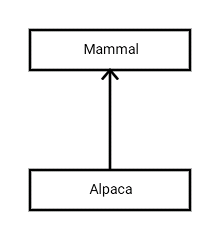
\includegraphics[width=\textwidth]{images/mammal}
    \end{columns}
\end{frame}

\begin{frame}
    \frametitle{Overview of Inheritance}
    \begin{columns}
    \column{0.7\textwidth}
    \begin{itemize}
        \item<2-> {\bf Inheritance} is when a subclass is created
            from a base class.
        \item<3-> In our example "Mammal" is the base class and 
            "Alpaca" is the subclass.
        \item<4-> A subclass takes on all of the attributes and methods of
            its base class.
        \item<5-> A subclass can override base class functions.
        \item<6-> A subclass has access to the base class's public and 
            protected members.
        \item<7-> A subclass is a more specific class than its base class.
    \end{itemize}
    
    \column{0.3\textwidth}
    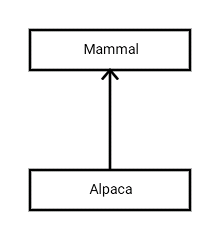
\includegraphics[width=\textwidth]{images/mammal}
    \end{columns}
\end{frame}

\begin{frame}[fragile]
    \frametitle{Inheritance Syntax}
    \begin{verbatim}
class Alpaca : public Mammal
{
    //class stuff here
};
    \end{verbatim}
    {\bf Visibility Specifiers}
    \begin{description}
        \item[{\tt public}]<2-> Public members of the base class become
            public members of the subclass
        \item[{\tt protected}]<3-> Public members of the base class become
            protected members of the subclass
        \item[{\tt private}]<4-> All members of the base class become private
            members of the subclass.
    \end{description}
\end{frame}

\begin{frame}
    \frametitle{Overriding Functions}
    \begin{itemize}
        \item<2-> If a function in the base class and subclass both have
            the same function signature (name and parameter types), 
            then the function is overridden.
        \item<3-> Invoking the function on an object of the subclass type
            will call the subclass version of the function.
        \item<4-> This is the beginning of the real power of inheritance.
        \item<5-> Let's play with this concept for a moment. 
            (inheritance.cpp example)
    \end{itemize}
\end{frame}

\section{Polymorphism}
\begin{frame}
    \frametitle{Overview of Polymorphism}
    \begin{itemize}
        \item<2-> {\bf Polymorphism} is a Greek-derived term which means "many forms".
        \item<3-> A reference to a subclass can be treated as a reference to
           a base class.
        \item<4-> The base class reference still behaves like the subclass!
        \item<5-> Allows us to program to the "general case", and further 
           modularize software development.
        \item<6-> This is the most powerful aspect of OOP, but it is the
           one of the most misunderstood and incorrectly used feature 
           of C++.
    \end{itemize}
\end{frame}

\begin{frame}
    \frametitle{The {\tt virtual} Specifier}
    \begin{itemize}
        \item<2-> A function can be specified as {\tt virtual} during its
          initial definition.
        \item<3-> A {\tt virtual} function is a function which has been
          marked for dynamic binding.
        \item<4-> Invoking a {\tt virtual} function on a base class pointer or
          reference will call the most-specific version of the function.
        \item<5-> This is what allows subclasses to change behaviors in code
          they never see!
        \item<6-> Unless you are really really really really certain you should
          do otherwise, member functions should be marked {\tt virtual}.
        \item<7-> Let's try it out. (polymorphism.cpp example)
    \end{itemize}
\end{frame}

\begin{frame}
    \frametitle{Polymorphism and Pointers}
    \begin{itemize}
        \item Polymorphism only works with pointers and references.
        \item A statically defined object cannot participate in polymorphism!
        \item This is why we generally use pointers when referring to objects.
    \end{itemize}
\end{frame}

\begin{frame}
    \frametitle{Up-casting and Down-casting}
    Consider the following:
    \par{\tt Mammal *m;}
    \par{\tt Alpaca *a1, *a2;}
    \par{\tt a1 = new Alpaca;}
    \begin{description}
        \item[Up-casting] - When a reference or pointer to a subclass is
            assigned to a reference or pointer of a base class.  In C++,
            up-casting is implicit.
            \par{\tt m = a1;}
        \item[Down-casting] - When a reference or pointer to a base class
            is converted to a reference or pointer of a subclass.  This 
            must be done explicitly. 
            \par{\tt a2 = (Alpaca*) m;}
    \end{description}
\end{frame}

\begin{frame}
    \frametitle{Pure Virtual Functions and Abstract Classes}
    \begin{itemize}
        \item<2-> A pure virtual function has no implementation in the base class.
        \item<3-> Such a function is created by assigning it the value of 
            nullptr at definition time:
            \par {\tt virtual void display()=0;}
        \item<4-> A class containing a pure virtual function is said to
            be an "abstract class".
        \item<5-> An abstract class cannot be instantiated. 
        \item<6-> Subclasses are required to override all pure virtual functions.
    \end{itemize}
\end{frame}

\section{Shapes Example}
\begin{frame}
    \frametitle{Program Specifications}
    \begin{itemize}
        \item Allow the user to move a cursor around on the canvas.
        \item Pressing the first letter of a shape begins drawing it.
        \item Move the cursor and press enter to set points in the shape.
        \item When the shape is complete, it will appear on the canvas.
    \end{itemize}
\end{frame}
\begin{frame}
    \frametitle{The Shapes Program Classes}
    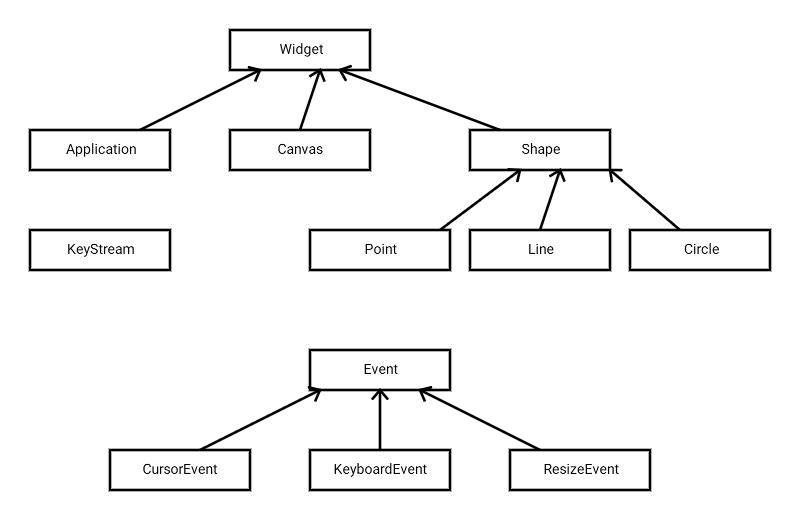
\includegraphics[height=0.8\textheight]{images/shapes}
\end{frame}
\end{document}


